\chapter{Background}
%Starting my final year project at the Electronic Vision(s) group, I soon realized the diversity of their research. 
The required knowledge to work in the field of neuromorphic computing is broad and manifold, ranging from the biological view of the human brain to electronic circuit laws further to machine learning algorithms. In the next sections, I will introduce the most important concepts and physical backgrounds upon which the presented research in this thesis is based on. Starting with deep learning and an overview of the biological neuron, the transition to neuron models, neuronal coding schemes and their training approaches will be made, before introducing neuromorphic \gls{bss2} platform 
\section{Deep Learning}
\label{deeplearning}
Deep learning is among the most useful and powerful tools machine learning has provided to the scientific community. Image or pattern recognition are in general hard to solve tasks for traditional computation concepts. Deep learning abstracts such task in terms of a hierarchy of concepts. Each concept is based upon a combination of simpler ones. Going down on a hypothetical ladder towards the easiest concept available, creates a deep structure with many layers. This is why it's called \emph{deep learning} (\cite{Goodfellow-et-al-2016}).

A popular example for deep learning is the \gls{mlp}, a deep feedforward network. As the name suggests, the information is forwarded from one layer to another. At each layer the input $\mathbf{x}$ is mapped to an output $\mathbf{y} = \gls{transfer}(\mathbf{x, \theta})$ by the transfer function \gls{transfer} and a set of parameters $\mathbf{\theta}$. The layer structure of such a network is inspired by biological neural networks and therefore such networks are often referred to as \glsfirst{ann}.

In machine learning, one discriminates between supervised, and unsupervised learning algorithms. Without a supervisor, an algorithm looks for structures and useful properties within the input data. Many machine learning algorithms are not supervised and try to observe the underlying probability distribution of the input data. In supervised learning, on the other side, each input vector $x$ is associated with a target vector $\hat{y}$. In this case, the algorithm is trained to predict a target for a given input.

Q: Überleitungssatz hier zu Supervised Training?

%Given the task to identify a picture of cat, any computer will have a hard time to map the essential information of the camera's sensor data to the class \textit{cat}. An \gls{ann} solves the problem by learning how to describe the raw data in terms of simpler representations and essentially by combining these simpler representations into a meaningful solution in the last layer - the output layer. The first layer is called input layer and all other layers in between are named hidden layers, since they are usually not visible from the outside.\\


\subsection{Supervised Training}
\label{supervisedtraining}
The training process of an \gls{ann} can be divided into a \emph{forward pass} where the output of all nodes is evaluated and a \emph{backward pass} which is responsible for the learning.

In the \textbf{forward pass}, the activation $\mathbf{a}^{(l)}$ of a layer $l$ yields
\begin{align}
\label{activation}
\mathbf{a}^{(l)} = W^{(l)} \, \mathbf{x}^{(l)} + \mathbf{b}^{(l)},
\end{align}
with the weight matrix $W^{(l)}$, the input $\mathbf{x}^{(l)}$ and the bias $\mathbf{b}^{(l)}$. The output value $\mathbf{y}^{(l)}$ of the layer is then given by the transfer function $\phi$, e.g. a sigmoid
\begin{equation}
\label{transferANN}
\mathbf{y}^{(l)} = \phi(\mathbf{a}^{(l)}) = \frac{1}{1 + e^{(-\beta x)}},
\end{equation}
with a slope parameter $\beta$. The choice of the transfer function is to a certain degree free. A \gls{relu}, a hyperbolic tangent ($\tanh$) or a sigmoid are among the most popular ones and are shown in \cref{deeplearning_activation_functions} for comparison.
However, it is important that the chosen function has a non-linear nature. With a linear transfer function any hidden layer structure becomes redundant, as the layers can be simply merged into a single one.

Depending on the task, the bias as well as an additional noise term can be vital: the individual biases for instance allows the network to adjust the dynamic range of each neuron and the injection of artificial noise can significantly increase the training performance. 

The same principle is then applied to all other layers to complete the forward pass, i.e. the result of the previous layer is the input for the current layer. The weight matrix $W^{\text{(l)}}$ connecting layer $l$ with $l-1$ has the appropriate shape to fit the number of input nodes $n^{\text{(l-1)}}_\text{nodes}$ and output nodes $n^{\text{(l)}}_\text{nodes}$.

\begin{figure}
	\begin{subfigure}[c]{0.5\textwidth}
		\centering
		\caption{}
		\inputpgf{figures}{deeplearning_activation_functions.pgf}
		\label{dltransfer}
	\end{subfigure}
	\begin{subfigure}[c]{0.5\textwidth}
		\centering
		\caption{}
		\inputpgf{figures}{deeplearning_activation_functions_derivative.pgf}	
		\label{dltransfergradient}
	\end{subfigure}
	\caption[]{(\subref{dltransfer}): Some of the most popular shapes for the transfer function are a \gls{relu}, $\tanh$ or sigmoid. (\ref{dltransfergradient}): Training with a linear function would not work, because the gradient is a constant and doesn't discriminate between different inputs. A non-linear transfer function is thus vital to the training. The \gls{relu} is, despite appearing to be a linear function, non-linear}
	\label{deeplearning_activation_functions}
\end{figure}

In deep learning the \textbf{backward pass} is almost always performed with \gls{sgd}, where a given loss function $\loss(\mathbf{\mathbf{x}, \hat{y}, \mathbf{\theta}})$ is minimized by moving along the negative gradient of the loss with respect to the network's parameters $\mathbf{\theta}$ (\cite{Goodfellow-et-al-2016}). The updated set  of parameters $\mathbf{\theta}'$ is then given by
\begin{equation}
\mathbf{\theta'} = \mathbf{\theta} - \eta \, \nabla\loss(\mathbf{\mathbf{x}, \hat{y}, \mathbf{\theta}}),
\label{stochasticgradientdescent}
\end{equation}
with the learning rate $\eta$. 

In combination with a cross-entropy loss function, the choice of the sigmoid transfer function becomes convenient when deriving the parameter changes. As an example the update of the weight matrices is computed in the next paragraphs.

In a first step, the derivative of the loss function in the output layer $l\equiv o$ is computed
\begin{equation}
\frac{\partial\mathcal{L}}{\partial \mathbf{y}^{(o)}} = 
- \frac{\hat{\mathbf{y}}}{\mathbf{y}^{(o)}} + 
\frac{1 - \hat{\mathbf{y}}}{1 - \mathbf{y}^{(o)}},
\end{equation}
with the output $\mathbf{y}^{(o)}$ and the target output $\hat{\mathbf{y}}$. The gradient of the loss can then be rewritten in terms of the error $\mathbf{e}^{(o)} = \hat{\mathbf{y}} - \mathbf{y}^{(o)}$ by using the derivative of the transfer function
\begin{align}
\frac{\partial \mathbf{y}^{(o)}}{\partial \mathbf{a}^{(o)}} = \frac{\partial \gls{transfer}(\mathbf{a}^{(o)})}{\partial \mathbf{a}^{(o)}} = \gls{transfer} (1 - \gls{transfer}),\\
\Rightarrow \quad \frac{\partial\mathcal{L}}{\partial \mathbf{a}^{(o)}} =
\frac{\partial\mathcal{L}}{\partial \mathbf{y}^{(o)}} 
\; \frac{\partial \mathbf{y}^{(o)}}{\partial \mathbf{a}^{(o)}} =
\hat{\mathbf{y}} - \mathbf{y}^{(o)} = \mathbf{e}^{(o)}.
\end{align}

According to \cref{stochasticgradientdescent}, the final update of the weight matrix is given by
\begin{equation}
\delta W^{(o)} = - \eta \frac{\partial \mathcal{L}}{\partial W^{(o)}} 
= - \eta \;
\frac{\partial\mathcal{L}}{\partial \mathbf{y}^{(o)}} \;
\frac{\partial \mathbf{a}^{(o)}}{\partial W^{(o)}}
= - \eta \, \left(\mathbf{e}^{(o)} \mathbf{x}^{(o),T}\right),
\label{backpropupdate}
\end{equation}

The computation for the hidden layer ($l\equiv h$) can be done in a similar fashion. Again, the gradient of the loss function is computed
\begin{equation}
\frac{\partial\mathcal{L}}{\partial \mathbf{a}^{(h)}} = \mathbf{e}^{(h)} \;
\frac{\partial \mathbf{y}^{(h)} }{\partial \mathbf{a}^{(h)}},
\end{equation}
and the error of the hidden layer $\mathbf{e}^{(h)}$ is propagated backwards as $\mathbf{e}^{(h)}=W^{(o),T}\mathbf{e}^{(o)}$ yielding a total update of
\begin{equation}
\delta W^{\text{(h)}} = - \eta \;
\left(W^{\text{(o)}T} \mathbf{e}^{(o)}\right) \;
\frac{\partial \mathbf{y}^{(h)} }{\partial \mathbf{a}^{(h)}} \; \mathbf{x}^{(h), T}.
\end{equation}

The backward propagation of the error is name giving and thus it is often referred to as \textit{backpropagation}. Despite the great performance for many deep learning tasks, the biological plausibility of propagating the error signal backward has been questioned ever since.

A simple but effective adjustment was suggested by \cite{lillicrap2016random} which is also known as \textit{feedback alignment}. Instead of the transpose of the feedforward weight matrix of the respective layer a fixed random matrix $B$ is chosen to propagate the error backward. Compared to the backpropagation variant from \cref{backpropupdate} the update in the hidden layer changes to
\begin{equation}
\delta W^{(h)} = - \eta \;
(B \mathbf{e}^{(o)}) \;
\frac{\partial \mathbf{y}^{(h)}}{\partial \mathbf{a}^{(h)}} \;
\mathbf{x}^{(h),T}
\end{equation}
The only constraints to $B$ are that $\mathbf{e}^{(o)T} W^{(o)} B \mathbf{e}^{(o)} > 0$ has to be fulfilled on average, meaning that geometrically, the new feedback signal $B \mathbf{e}^{(o)}$ for the hidden layer lies within $90^{\circ}$ of the one used by backprogation, $W^{\text{(o)}T} \mathbf{e}^{(o)}$.

Überleitung zu biologischem neuron hier?

\section{The Biological Neuron}

Biological neural networks have been a great inspiration for deep learning algorithms and \glspl{ann}. It is estimated that the human brain contains around $10^{11}$ neurons of different shape, size and functions (\cite{numberofneurons}). By the use of \emph{synapses}, neurons create complex network structures throughout the brain. Usually a neuron has up to $10^4$ \emph{postsynaptic} partners. The connections vary from dense clusters with nearby neurons to linking distant brain regions with each other. 

The intercommunication is established by the use of short electrical pulses (spikes) and neurotransmitters. At most synapses, a small physical gap separates the neurons from each other. An electrical pulse of the \emph{presynaptic} neuron releases various neurotransmitter to overcome this synaptic cleft and once a transmitter has docked to a corresponding receptor on the other side, activated ion channels convert the chemical transmission back into an electrical signal. Depending on the type of neurotransmitters the excitation  can be excitatory or inhibitory. According to Dale's principle a presynaptic neuron releases always the same type of neurotransmitter. To that end, a neuron's output is either inhibitory or excitatory but not both. The input, on the other side, is not restricted to a single type of excitation, as various presynaptic partners can be connected.

On the postsynaptic side, the inputs of all presynaptic partners are then gathered by the \emph{dendrites} before they are forwarded to the \emph{soma} where the information is processed (c.f. \cref{biosynapse}). In particular, the soma integrates the currents induced by the input spikes, which can be tracked by measuring the course of the soma's membrane potential. The impact of each spike corresponds to a \gls{psp}. Once a certain threshold potential is reached, a mechanism gets triggered that initiates a fire response, the so-called action potential or spike. Once a spike has been fired, the neuron's membrane becomes hyperpolarized and decrease even below the resting potential as shown in \cref{actionpotential}. The neuron is in a so called \emph{refractory state} and due to the ongoing hyperpolarization it is hard but not impossible to fire. The action potentials are then relayed by the axon to its connected partners and the described course of communication starts over. 

\begin{figure}
	\begin{subfigure}{0.5\textwidth}
		\centering
		\caption{}
		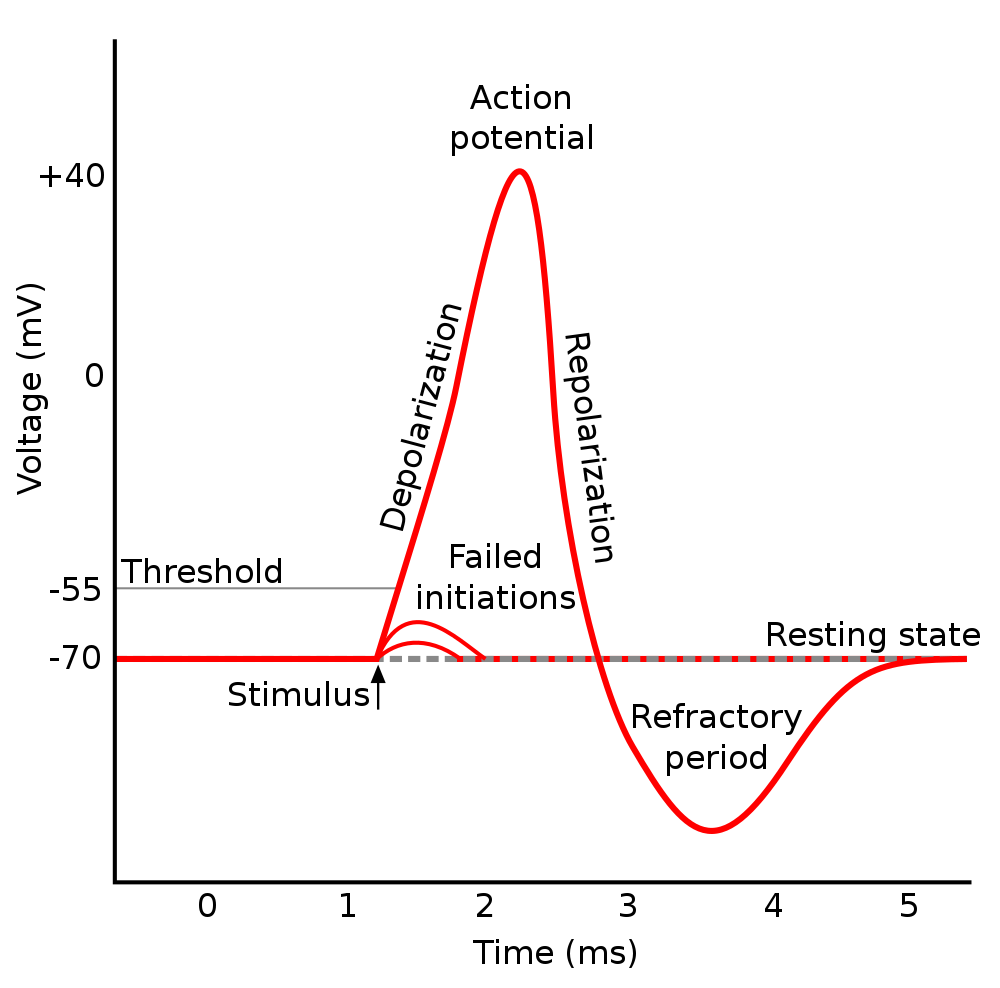
\includegraphics[width=0.8\linewidth, valign=t]{figures/action_potential.png}
		\label{actionpotential}
	\end{subfigure}
	\begin{subfigure}{0.5\textwidth}
		\centering
		\caption{}
		\vspace{0.5cm}
		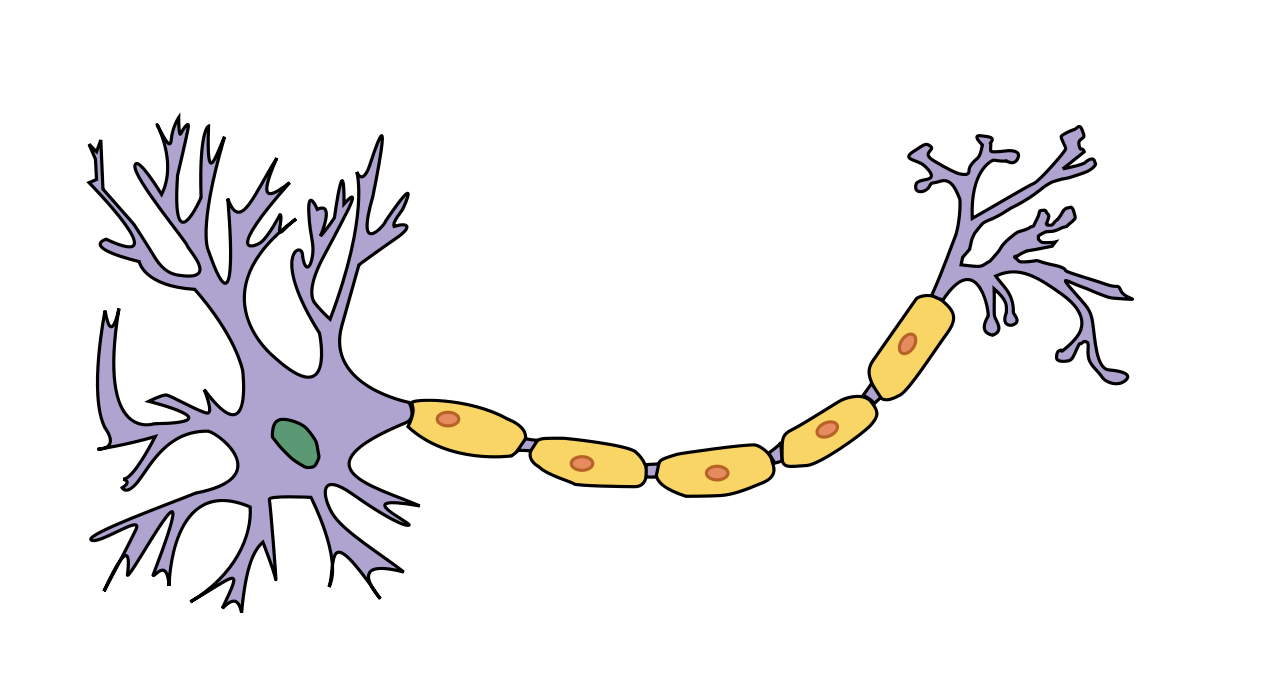
\includegraphics[width=\linewidth, valign=t]{figures/neuron_model.png}
		\vspace{1.5cm}	
		\label{biosynapse}
	\end{subfigure}
	\caption[Schematics of an action potential and a biological neuron]{Schematics of a biological neuron and an action potential: \textbf{(\subref{actionpotential})} The response of neuron after exceeding the threshold is called action potential. After a phase of depolarization, the membrane repolarizes and enters the refractory state.\textbf{(\subref{biosynapse})} Schematics of a biological neuron can be split into three main functional parts: the dendrites which are responsible to collect all inputs, the soma integrates the evoked \glspl{psp} and eventually triggers a fire response and the axon relays the fire responses to other neurons.}
	\label{biologicalneuron}

\end{figure}

Over time the unbalanced ion concentration in and outside the membrane is restored by the membranes permeability and additional ion pumps. In the equilibrated state, the membrane potential is then referred to as the \emph{resting potential}. The neurotransmitters are recycled as well. Otherwise, if their resources were depleted and heavily used synapses would be quickly silenced.

A wide-spread assumption in the field of neuroscience is that the exact shape of a spike doesn't carry any relevant information and therefore all spikes can be modeled by a stereotypical shape. The communication between neurons is then encoded in the frequency (\emph{rate coding}) or timing (\emph{time coding}) of exciting and inhibiting spikes. A more detailed description of neural coding schemes is presented in section \ref{neuralcoding}. However, recent research has already suggested that the variate of action potential contains vital information (\cite{debanne2013mechanisms}).

The brain's ability to continuously change the topology of its synaptic wiring, to create new synapses, to alter the chemical properties of the synaptic receptors or to simply strengthen and weaken the synaptic efficacy, allows it to learn and react as a response to stimulation and even brain damage.

One way of learning and forming memory is known as synaptic plasticity where the synaptic strength is changed over time. According to Hebb's theory ``neurons that fire together wire together" (\cite{hebb1949organization}). An experimental proof of such activity-dependent plasticity was found by \cite{bliss1973long}, where they discovered that a short but high frequency stimulation lead to a long lasting change in the synapse's efficacy. This is also referred to as \gls{ltp}. Reducing the stimulus to a low frequency, on the other hand, resulted in the opposite effect: \gls{ltd}. In combination they can carve out certain region in the brain which is related  to a stimulus and thereby create memory. 

A better understanding of \gls{ltp} and \gls{ltd} was provided by the introduction of \gls{stdp}. \gls{stdp} shows in principle that a presynaptic activity just before a postsynaptic response leads to an increase synpatic strength and if presynaptic activity occurs right after the postsynaptic one, it results in the inverse effect (\cite{poo98stdp}). 

It is worth mentioning that synaptic plasticity between two neurons can also be induced by activity of an independent pathway. 

In the next section a popular and practicable neuron model is presented 

Developing biologically inspired and plausible learning algorithms is a dedicated goal in the field of modern neuroscience. In the next section a practicable neuron model is presented, which is the basis of the experimental part in this thesis.

\section{\gls{lif} Model}

An early but successful description of the biological neuron dynamics was accomplished by the \gls{lif} neuron, first described by \cite{lapicque1907recherches}. Despite some strong simplifications, the main dynamics of the membrane potential are well described by the model and it thus has been a popular and portable choice for neuromorphic hardware implementations.

In biology, the observation of similar shaped individual action potentials lead to the assumption that the shape of an spike does not transport any information. The \gls{lif} model is based upon this theory and thus every spike can be replaced by a stereotypical shape.

Another observation in biology is, that neurons vary much in their shape and size fulfilling different functions. The spatial component plays an important role for the dynamics of a neuron. For instance, the strategic positioning of certain excitatory or inhibitory inputs on the dendrites, either closely or further away from the soma, give rise to non-linear behavior in the course of the membrane potential. However, a extensive spatial dependency is difficult and costly to implement in a model. Therefore, the \gls{lif} neuron neglects the topology of the neuron and is approximated as a point-like integrator. 

In the model, the incoming spike trains $S_j(t)$ from various presynaptic partners $j$ are described by a series of spikes $s$ at times $t_j^{(s)}$
\begin{equation}
S_j(t) = \sum_s \delta(t - t_j^{(s)}),
\end{equation}
with the $\delta$-function denoted as $\delta$. 

Each spike of the input spike train evokes a \gls{psp}. The impact of the \glspl{psp} depends on the individual synaptic weights $w_j$. For simplicity, the excitatory or inhibitory nature of the synapses is encoded by a sign in the synaptic weight as well. Summing over all input sources yields a total synaptic input current that is seen by the postsynpatic neuron
\begin{equation}
\gls{isyn}(t) = \sum_j w_j \left(\epsilon \ast S_j(t)\right),
\label{synpatic_input}
\end{equation}
with an exponential kernel $\epsilon$ describing the shape of the \gls{psp}. Popular choices for the kernel are single or double-exponentials
\begin{align}
\epsilon_\text{double}(t) 	&= \left(\epsilon_\text{rise} \ast \epsilon_\text{fall}\right)(t) \\
							&=\frac{1}{\mathcal{N}}\exp \left(-\frac{t}{\tau_\text{rise}} \right)  \ast \exp \left(-\frac{t}{\tau_\text{fall}} \right) 
\label{exponentialkernels)}
\end{align}
with a rising and falling temporal constant $\tau_\text{rise}$ respectively $\tau_\text{fall}$ and a norming constant $\mathcal{N}$. As the rising constant goes to zero $\tau_\text{rise} \rightarrow 0$ the double exponential turns into a single exponential kernel $\epsilon_\text{single} = \epsilon_\text{fall}$.

The membrane potential \gls{v_mem} changes with the continuous synaptic input causing an unbalanced ion concentration inside the membrane. Passive as well as active processes are permanently restoring the membrane potential back to its equilibrium state which is associated with the resting potential \gls{v_leak}. In the \gls{lif} model, the temporal scale of these restoring processes defined by the membranes capacitance $C_\text{m}$ and the leakage conductance $g_\text{leak}$ yielding the membrane's time constant $\gls{tau_m} = \frac{C_\text{m}}{g_\text{leak}}$. The dynamics of membrane are then given by a single differential equation
\begin{align}
\label{lifeq}
C_{\text{m}} \frac{d\gls{v_mem}}{dt} &= -g_{\text{leak}} (\gls{v_mem} - \gls{v_leak}) + \gls{isyn}.
\end{align}

As for a biological neuron, the postsynaptic \gls{lif} neuron $i$ triggers a spike once a certain threshold \gls{thres} is crossed following the condition
\begin{equation}
V_{\text{m}, i}\left(t_i^{(s)}\right) \ge \gls{thres} \Leftrightarrow \text{neuron i fires at time } t_i^{(s)}.
\end{equation}

Then the membrane is set to a reset potential \gls{v_reset} where it remains unchanged for a refractory period of \gls{refrac}
\begin{equation}
V_{\text{m}, i}(t) = \gls{v_reset} \quad \forall t \in \left(t_i^{(s)}, t_i^{(s)} + \gls{refrac}\right].
\end{equation}
Unlike for its biological counterpart, the modeled neuron cannot spike during the refractory period.

A \gls{lif} neuron doesn't keep track of any previous spikes once a spike is released, given that the time constant of the synaptic input is shorter than the one of the membrane potential, in particular if $\tau_\text{m} > \tau_\text{fall}$. These limitations make it impossible for the model to correctly describe neuronal behavior such as spike bursts.

The constraints of the \gls{lif} neuron led to a demand of a more detailed model, namely the \glsfirst{adex} model, which is an extension to the \gls{lif} model featuring an additional adaption state variable that provides post-spike memory to the membrane. Depending on the sign of the adaption, the in a neuron is either inhibited or engaged to fire again after having spiked at least once (see \cref{lifvsadex}).

%Apart from the additional state variable the \gls{adex} neuron features a positive exponential voltage feedback. on the other hand, enables the neuron to have a more complex behavior in the (\gls{v_mem}, w?) phase space.

\begin{figure}
	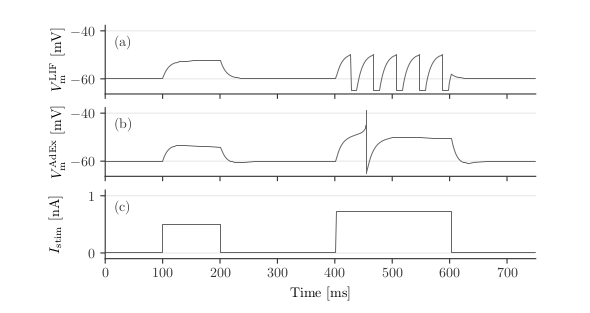
\includegraphics[width=\linewidth]{figures/LIFvsAdEx.png}
	\caption{Difference of membrane dynamics between a \gls{lif} and \gls{adex} neuron, given the same synpatic input. Figure taken from Stradmann, 2019}
	\label{lifvsadex}
\end{figure}


\section{Neural Coding with \glspl{snn}}
\label{neuralcoding}
Neuromorphic hardware uses spikes to transmit data from one neuron to another and the mapping function is represented by the modeled neuron (e.g. the \gls{lif} neuron). In terms of deep learning, such networks are called \glspl{snn}. In the biological introduction (\cref{biologicalneuron}) two methods of neural coding have already been mentioned: \emph{temporal coding} and \emph{rate coding}. The different types of neural coding require each an adapted training method for \glspl{snn}.

\textbf{Rate coding} for instance uses a high number of spikes to establish a certain firing rate of the neuron. The information is not encoded in a single spike or the time interval between two spikes but in a number of spikes within a certain period defining the \textit{rate}. 

Rate coding can be treated similar to glspl{ann} and thus classical training methods such as gradient descent will work just fine. 

\textbf{Temporal coding} on the other hand focuses on the \gls{isi}. This type of coding is more exposed to noise but for some applications it might be simply too slow to establish a certain fire rate first. The \gls{isi} on the other can be adapted quickly. 

However, for temporal or sparse coding the gradient descent approach doesn't work since the binary nature of spikes make the neurons output non-differentiable. Recent research has suggested workarounds for this problem, e.g. in \cite{zenke2018superspike} a surrogate gradient descent implementation for \glspl{snn} called \emph{SuperSpike} is presented.


Todo: a bit more in this section!

%When only a small set of all available neurons is used to describe an input pattern, its called \textbf{sparse coding}.\\


\subsection{Gradient Descent for \glspl{snn}}

Spikes can encode information in various ways. One of them is rate coding, where a certain fire rate is established and the rate itself contains the information. Other then for sparse or spike time dependent coding, the information of a single spike is not relevant. The transfer function of the neuron contains still an activation jump. At a certain input rate the neuron will suddenly start to fire. This can be smoothen out by setting the leak and threshold potential close to each other and by adding Poisson distributed noise spikes. In combination this will establish a certain equilibrium fire rate given there is no further input. Now, by applying inhibitory input the fire rate will go down. Excitatory input causes the opposite.

The above described method turns a \gls{snn} almost into an \gls{ann}. However, The forward pass is still not performed perfectly by a powerful GPU but by a noisy and power-efficient analog core. Noise is essential for learning algorithms to perform and is often artificially injected for \glspl{ann}. This is not necessary for the \gls{bss2} platform. In the experiment section, gradient descent with feedback alignment is conducted on the \gls{dls}.


\subsection{Novel Training Methods for \glspl{snn}}
\label{superspike}


Until now, only few people have successfully trained \glspl{snn} with hidden units. The main issue arises from the non-differentiable dynamics of spikes. A promising approach was proposed by \cite{zenke2018superspike} with SuperSpike. Similar to the training of \glspl{ann} the learning process can be split up into a forward and backward pass. 

The \textbf{forward pass} only changes slightly compared to \glspl{ann}. Instead of a continuous input and output one speaks of presynaptic spike train $S_j$ and a postsynaptic spike train $S_i$. Note that the choice of the index $j$ and $i$ indicate if, from the perspective of a neuron, the spike is of presynaptic or postsynaptic origin. The transfer function $\phi$ is replaced by the dynamics of the \gls{lif} neuron.

%Todo: "surrogate gradient" is not really introduced but just used -> fix this
%Todo: spike train formalism (maybe in biological part with synapses, etc. ), presynaptic/postsynpatic 
%Todo: axonal delay is not considered for the application of the hardware
%Todo: auxilary function: threshold! -> f(x) = x/(1 + |x|) and f'(x) (1 + |x|)-2 => $\sigma'(U_i) = (1+|U_i - \vartheta|)^{-2}$

As stated in section \ref{trainingANN}, most training approaches involve the optimization of a certain loss function $\mathcal{L(\mathbf{\theta)}}$ that depends on the network's parameters $\mathbf{\theta}$. In the \textbf{backward pass} of the SuperSpike formalism the von Rossum distance (\cite{rossum01novel}) of a target spike train $\hat{S}_i$ and the output spike train $S_i$ is chosen, c.f. \cite{zenke2018superspike},
\begin{equation}
\label{vonrossumdistance}
\mathcal{L} = \frac{1}{2} \int^t_{-\infty}dt' \left[\left(\alpha \ast \hat{S}_i - \alpha \ast S_i \right)(t')\right]^2
\end{equation}
where $\alpha$ is a smooth double exponential convolution kernel. The computation of the gradient for \ref{vonrossumdistance} with respect to $\mathbf{\theta}$ requires the derivative of a spike train $\nicefrac{\partial{S_i}}{\partial{w_{ij}}}$ which is undefined for the time of a spike. 

SuperSpike circumvents this issue by rendering the spike train with a smooth auxiliary function $\sigma(V)$ of the membrane potential $V$ and thus the ill defined gradient of the spike train can be replaced by a surrogate derivative $\sigma'(V)$
\begin{equation}
\frac{\partial S_i}{\partial w_{ij}} \quad \rightarrow \quad \sigma'(V_i)\frac{\partial V_i}{\partial w_{ij}}.
\end{equation}

The choice of the auxiliary function $\sigma$ the therefore implied surrogate derivatives is to a certain degree free. SuperSpike suggest a deterministic approach with the negative side of a fast sigmoid $\sigma(V) = \frac{V - \vartheta}{1 + |V - \vartheta|}$. The surrogate partial derivative yields $\sigma'(V) = \left(1 + |V - \vartheta|\right)^{-2}$. Another common choices are pieces-wise linear or exponential approaches.

At a first glance, it appears that the problem has just been moved to computing the partial gradient of the membrane potential instead. When the potential $V_i$ is formulated as a spike response model for \gls{lif} neuron (Gerstner et al., 2014) it again depends on the output spike train $S_i$. However, under the assumption of a low output rate the gradient can be approximated by $\frac{\partial U_i}{\partial w_{ij}} \approx (\epsilon \ast S_j)$ with $\epsilon$ another double-exponential kernel corresponding to the shape of a spike. Plugging in the approximation and the formulation of the gradient as a surrogate gradient yields

\begin{equation}
\label{superspikeweightupdateeq}
\frac{\partial w_{ij}}{\partial t} = \eta \int_{-\infty}^{t} dt'
\underbrace{\left(\alpha \ast (\hat{S}_i - S_i)\right)}_{= e^{(o)}_k \; \text{(Error)}} 
\; \alpha \ast 
\Big(\underbrace{\sigma'(U_i)}_{\text{Pre}} 
\underbrace{\left(\epsilon \ast S_j\right)}_{\text{Post}}\Big)
\end{equation}
with $\eta$ the learning rate. The formulation for the hidden layer is similar with the only exception of how the error is calculated. Inspired from the popular backpropgation method the error signal of the $i \text{-th}$ hidden unit $e^{(h)}_i$ is propagate backwards as a weighted sum over the all output error signal $e^{(h)}_i = \sum_{k} w_{ik} e^{(o)}_k$ with $w_{ik}$ the feed forward weights between the hidden and the output layer. A feedback alignment oriented approach with random weights is also possible. This formalism can be easily adapted for multiple hidden layers too.


%ToDo: Literatur Book zu Deep Learning (siehe downloads UniRechner)
%
%Überleitung zu rate coding vs sparse coding (maybe read again SuperSpike17/19 first))
%A \gls{snn} offers many advantages compared to a classical \gls{ann}. On of the major differences is that sparse coding allows the user to compress a lot of information into a single spike. Also not spiking at a sppecifencodes information.  This efficient way of transporting information makes \glspl{snn} a contender for any energy sensitive form of computing. More importantly it also opens up the doors to understanding spike-based computing better and thus also the way the human brain works.




\section{Neuromorphic Hardware}

Certain tasks, such as pattern recognition, are quite difficult to solve with traditional computing methods.  Biologically inspired computing has provided a range of efficient approaches to successfully tackle these problems. In the same way, biology has also been the key inspiration for a new \emph{neuromorphic} hardware design. As it's paradigm, neuromorphic hardware is designed to be robust to malfunctioning sectors, energy efficient and adaptive. 

As of today, several well known tech companies have launched their own neuromorphic platform. IBM started to work on \emph{TrueNorth} in 2008, Intel presented the \emph{Loihi} chip in 2018 and Google started selling the \emph{Coral} dev-board in 2019. But even before neuromorphic hardware caught the attention of the big industry names, academic projects have already been started. Among others, the EU's Human Brain Project (HBP) funds two promising approaches: \emph{SpiNNaker}, a digital based neuromorphic supercomputer located in Manchester and \emph{\gls{bss}}, a mixed-signal accelerated emulation for spiking neural networks based in Heidelberg.

The \gls{bss2} platform is based upon a complete redesign of the \gls{hicann} chip from its predecessor \gls{bss1}. By using a smaller manufacturing process (\SI{65}{\nano \m} instead of \SI{180}{\nano \m}) several new features could be included on the new core - the \gls{hx}. The analog mixed-signal neuromorphic chip with 512 \gls{adex} neuron circuits and 256 possible synaptic connections per neuron is especially designed to investigate various on-chip plasticity algorithms. Therefore it features two \glspl{ppu}, on-chip event routing and the HAGEN extension. The latter is an early realization of a neuromorphic system which basically implements analog matrix multiplication on-chip (\cite{schemmel2020accelerated}).

The new features have been tested step by step on smaller prototype systems, e.g. on the \gls{dls} the newly designed \gls{lif} neuron was tested. To avoid unnecessary costs, the size was reduced to $32$ neurons and a corresponding $32 \times 32$ synapse array allows all to all connectivity. Besides the Hagen extension and the \gls{adex} neuron, the main features of the \gls{bss2} platform, such as the \gls{ppu}, are already available on the prototyped versions.

%The experiments conducted within this thesis are done either on the \gls{hx} or the \gls{dls}. In the following section the individual parts of the chip are discussed.
%The manufacturing has been outsourced to the Taiwan Semiconductor Manufacturing Company (TSMC) using a standardized $65 \si{nm}$ low-power and low-leakage CMOS technology.

%refs: ibm http://www.research.ibm.com/articles/brain-chip.shtml
% coral board:
% Loihi:

\subsection{Architecture of \gls{bss2}}

The design of the \gls{hx} chip can be divided into an \emph{analogue} and \emph{digital} core (c.f. figure \ref{hxstructure}). 
\begin{figure}
	\begin{subfigure}[c]{0.5\textwidth}
		\centering
		\caption{}
		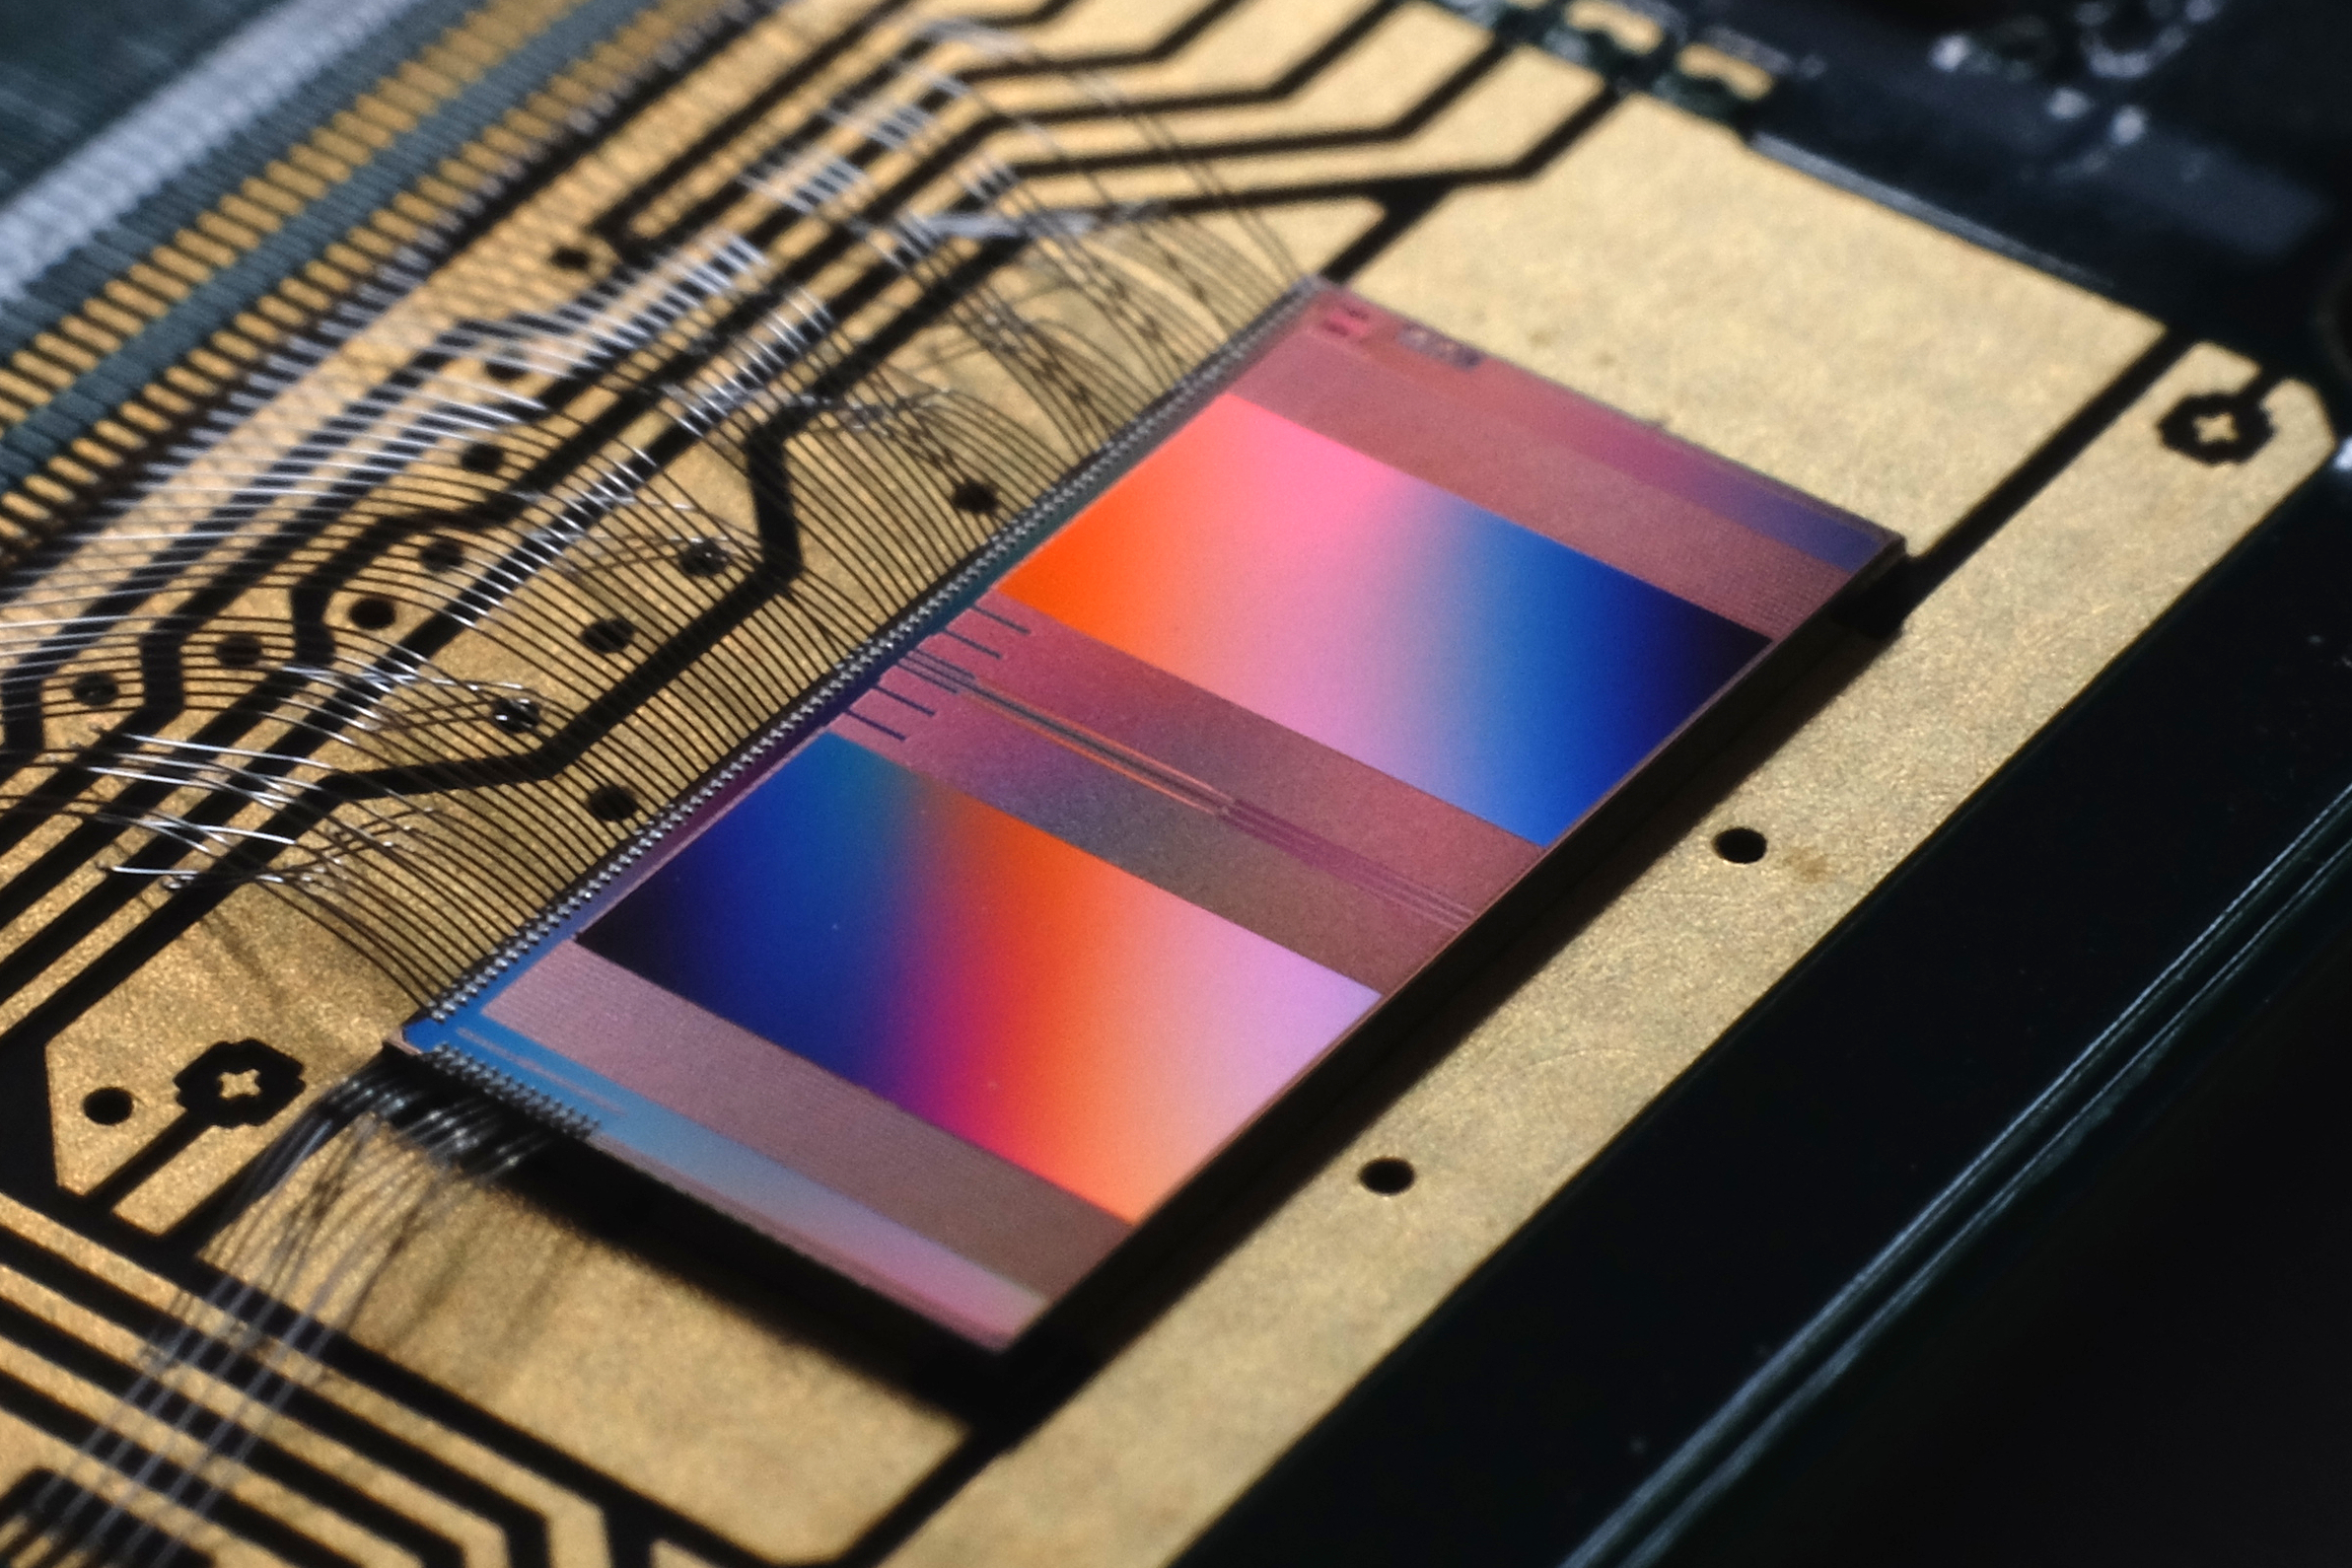
\includegraphics[width=\textwidth]{figures/HXcloseup.JPG}
		\label{hxcloseup}
	\end{subfigure}	
	\begin{subfigure}[c]{0.5\textwidth}
		\centering
		\caption{}
		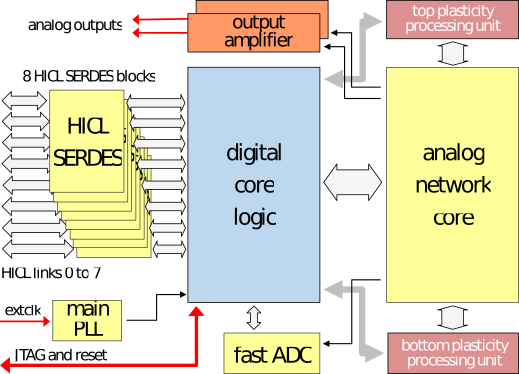
\includegraphics[width=\textwidth]{figures/g3418.png}
		\label{hxstructure}
	\end{subfigure}
	\caption{The \gls{bss2} platform uses a mixed-signal neuromorphic chip. (\subref{hxcloseup}): Close-up of the bonded \gls{hx} chip, picture taken by Müller, 2020. (\subref{hxstructure}): Overview of the digital and analog core of the \gls{bss2}.   . Figure taken from \cite{schemmel2017nmda}}
\end{figure}

The analogue core contains the physical implementation of the \gls{lif} and the \gls{adex} neuron model respectively (c.f. \cite{aamir2018dls2neuron} and \cite{aamir2018mixed}). The biological time constants of neurons and synapses are usually in the order of 1 to 100 milliseconds. The \textit{in-silico} implementation of the neuron models create a temporal speed-up compared to their \textit{in-vivo} counterpart, leading to on-chip time constants of a few microseconds. This acceleration is possible by the supra-threshold dynamics of CMOS transistors. 

% STOPPED HERE:

The analog neuron model parameters in both chips are tunable by setting bias currents over an 10 bit \gls{dac} \cite{hock13analogmemory}, which allows to control and adjusted each neuron individually. The 8-bit spike counter of the \gls{dls} (one per neuron) has been upgraded to a 10 bit counter in the \gls{hx}. 

The wiring of the neurons is achieve by a grid of $512 \times 256$ synapses ($32 \times 32$ on the prototypes). Each synapse has access to a 16 bit local \gls{sram} to store a 6-bit weight and information about the presynaptic connections. In addition, two correlation sensors per synapse (causal and anti-causal) record \gls{stdp} traces and store them in dedicated capacitors. These analog observables can then be processed by a \gls{ppu} via an \gls{cadc}. The readout is performed per row and thus a total of 1024 \gls{cadc} channels (one channel per correlation sensor per synapse) can be accessed by the \gls{ppu}. The access to further observables such as the membrane potential are also realized by the \gls{cadc}. This feature has not been available on the prototype revisions such as the \gls{dls} and opens up new possibilities for plasticity rules on \gls{hx}.

A highly accelerated analog system requires a fast computation of any plasticity rule. To provide sufficient computational power, the chip is equipped with two \glspl{ppu}, each containing a general-purpose unit that is extended with a special function unit implementing \gls{simd} operations. The special function unit has vector-wise access to the synapse array as well as to the results of the \gls{cadc} and will be further referred to as \emph{vector unit}.

As an additional debugging and observation tool, a \gls{madc} can be accessed from the digital core to readout any available analog observables.

Apart from the spike counters, the digital neuron back end registers any spiking event. Such an event may also come from one of the noise generators or \glspl{ppu} as well as from an external source. Once a spike has been registered in the digital neuron back end, it is routed back into the synapse array accordingly. 

The communication with an external host is streamed out to the controlling Field Programmable Gate Array (FPGA). The existing FPGA solution developed for \gls{bss1} was simply transfered to \gls{bss2}.

The link between chip and external host is established via an \gls{fpga} accessing eight serial Low Voltage Differential Signaling (LVDS) links. This interface handles read/write instructions and manages spike event data in both directions. %The FPGA grants access for the PPU to greater memory storages than the one provided on-chip. Access to large training datasets is vital for most learning tasks.